\documentclass[12pt]{article}

\usepackage{fancyhdr}
\usepackage{lastpage}
\usepackage{float}
\usepackage{tikz}
\usepackage{amsmath}
\usepackage{pgfplots}
\usepackage{multirow}
\usepackage{caption}
\usepackage{amssymb}
\usepackage{subcaption}
\usepackage{listings}
\usepackage{diagbox}
\usepackage{longtable}
\usetikzlibrary{automata,positioning,arrows}
\usepackage[top=2.2in, left=0.75in,right=0.75in,headsep=1mm,footskip=.5in]{geometry}

\usepackage{array}
\usepackage{multirow}
\usepackage{float}
\usepackage{booktabs}


\usepackage{ifthen}
\newboolean{showsolutions}
\setboolean{showsolutions}{false} % change to show/hide solutions.
\ifthenelse{\boolean{showsolutions}}{%
  % When showing solutions
  \newenvironment{solution}
    {\par\noindent\textbf{\textcolor{blue}{Solution:}}\par}
    {}
}{%
  % When hiding solutions: just ignore content
  \newenvironment{solution}
    {\expandafter\ignorespaces}
    {}
}
\usepackage{xcolor}


\makeatletter
\newcommand\cdotfill{%
    \leavevmode\cleaders\hb@xt@.44em{\hss$.$\hss}\hfill\kern\z@
}
\makeatother

% Custom line background command
\definecolor{lightgray}{gray}{0.95}
\definecolor{white}{gray}{1.0}
\makeatletter
\lst@AddToHook{OnLine}{%
  \ifnum\value{lstnumber}=0\relax\else
    \ifodd\value{lstnumber}
      \color{white}\lst@basicstyle\colorbox{white}{\strut}
    \else
      \color{lightgray}\lst@basicstyle\colorbox{lightgray}{\strut}
    \fi
  \fi
}
\makeatother

\usepackage{algorithm}
\usepackage{algpseudocode}

\pagestyle{fancy}
\let\headrule\empty
\let\footrule\empty
\rhead{\hrule}
\chead{\hrule}
\lhead{\hrule}
\lfoot{CSC\,263\,H1, Fall 2025}
\cfoot{Page \thepage\space of \pageref{LastPage}}
    \rfoot{Quiz 2}

\DeclareMathOperator*{\argmax}{arg\,max}
\DeclareMathOperator*{\argmin}{arg\,min}

\begin{document}

\newcommand{\checkbox}[1][Option]{
  \begin{tikzpicture}[baseline=0]
    \node[draw=black, minimum size = 0.5cm] (s) {};
    \node[right = 0cm of s, align = left]{#1};
  \end{tikzpicture}%
}

\newcommand{\checkboxmath}[1][Option]{
  \begin{tikzpicture}[baseline=0]
    \node[draw=black, minimum size = 0.5cm] (s) {};
    \node[right = 0cm of s, yshift=-1mm, align = left]{#1};
  \end{tikzpicture}%
}

\newcommand{\points}[1][0]{
  {[#1 pts]}
}

\newcommand{\choice}[1][Option]{
  \begin{tikzpicture}[baseline=0]
    \node[circle, draw=black, minimum size = 0.5cm] (s) {};
    \node[right = 0cm of s, yshift=-0.7mm, align = left]{#1};
  \end{tikzpicture}%
}

\newcommand{\tf}{
  \\~\\
  
\begin{tikzpicture}
    \node[circle, draw=black, minimum size = 0.5cm] at (0,0) (t) {};
    \node[right = 0cm of t, yshift=-1mm, align = left]{True};


    \node[circle, draw=black, minimum size = 0.5cm] at (4,0) (f) {};
    \node[right = 0cm of f, yshift=-1mm, align = left]{False};
  \end{tikzpicture}%
}

\newcommand{\numbox}[1][5em]{
  \begin{tabular}{|c|}         \hline \hspace{#1} \\ \\ \\ \hline     \end{tabular}
}

\newcommand{\fractional}[1][]{
  #1 \begin{tabular}{|c|}         \hline \hspace{5em} \\ \\ \\ \hline     \end{tabular} $\Bigg/$ \begin{tabular}{|c|}         \hline \hspace{5em} \\ \\ \\ \hline     \end{tabular}
}

\newcommand{\tableanswer}[1][Title]{
  \begin{tabular}{|l|}         \hline #1 \\ \hspace{5em} \\ \\ \hline     \end{tabular}%
}

\newcommand{\blank}[1][2cm]{
\underline{\hspace{#1}}
}

\newcommand{\infobox}[1][Title]{
  \noindent #1
  \begin{table}[H]
    \begin{tabular}{|c|c|c|c|c|c|c|c|c|c|c|c|c|c|c|c|c|}
      \hline
      \hspace{1.2em}\; & \hspace{1.2em}\; & \hspace{1.2em}\; & \hspace{1.2em}\; & \hspace{1.2em}\; & \hspace{1.2em}\; & \hspace{1.2em}\; & \hspace{1.2em}\; & \hspace{1.2em}\; & \hspace{1.2em}\; & \hspace{1.2em}\; & \hspace{1.2em}\; & \hspace{1.2em}\; & \hspace{1.2em}\; & \hspace{1.2em}\; & \hspace{1.2em}\; & \hspace{1.2em}\; \\
      \hspace{1.2em}\; & \hspace{1.2em}\; & \hspace{1.2em}\; & \hspace{1.2em}\; & \hspace{1.2em}\; & \hspace{1.2em}\; & \hspace{1.2em}\; & \hspace{1.2em}\; & \hspace{1.2em}\; & \hspace{1.2em}\; & \hspace{1.2em}\; & \hspace{1.2em}\; & \hspace{1.2em}\; & \hspace{1.2em}\; & \hspace{1.2em}\; & \hspace{1.2em}\; & \hspace{1.2em}\; \\\hline
    \end{tabular}%
  \end{table}
}

\newcommand{\spacer}[]{
  \vspace{5mm}\\
}

\newcommand{\hspacer}[]{\\
}

\begin{center}\large
  UNIVERSITY OF TORONTO\\
  Faculty of Arts and Science\\[1.75ex]
  Department of Computer Science\\[1.75ex]
  \textbf{Quiz 2} \\
  \textbf{{CSC\,263\,H1}}
\end{center}

\infobox[\textbf{First Name:}]
\infobox[\textbf{Last Name:}]

\noindent \textbf{Student \# (9 or 10 digits):} \begin{table}[H]
    \begin{tabular}{|c|c|c|c|c|c|c|c|c|c|}
      \hline
      \hspace{1.2em}\; & \hspace{1.2em}\; & \hspace{1.2em}\; & \hspace{1.2em}\; & \hspace{1.2em}\; & \hspace{1.2em}\; & \hspace{1.2em}\; & \hspace{1.2em}\; & \hspace{1.2em}\; & \hspace{1.2em}\; \\
      \hspace{1.2em}\; & \hspace{1.2em}\; & \hspace{1.2em}\; & \hspace{1.2em}\; & \hspace{1.2em}\; & \hspace{1.2em}\; & \hspace{1.2em}\; & \hspace{1.2em}\; & \hspace{1.2em}\; & \hspace{1.2em}\;\\\hline
    \end{tabular}%
  \end{table}
\noindent \textbf{UTORid (e.g. \texttt{gummalur}):} \begin{table}[H]
    \begin{tabular}{|c|c|c|c|c|c|c|c|}
      \hline
      \hspace{1.2em}\; & \hspace{1.2em}\; & \hspace{1.2em}\; & \hspace{1.2em}\; & \hspace{1.2em}\; & \hspace{1.2em}\; & \hspace{1.2em}\; & \hspace{1.2em}\; \\
      \hspace{1.2em}\; & \hspace{1.2em}\; & \hspace{1.2em}\; & \hspace{1.2em}\; & \hspace{1.2em}\; & \hspace{1.2em}\; & \hspace{1.2em}\; & \hspace{1.2em}\;\\\hline
    \end{tabular}%
  \end{table}
\noindent \textbf{Duration:}\cdotfill {50 minutes}\\
\textbf{Instructor:}\cdotfill Chandra Gummaluru\\
\textbf{Weight:}\cdotfill 10\% \\
%\textbf{Aids Allowed:}
%\begin{enumerate}
%    \item[(1)] Non-Programmable Calculator 
%\end{enumerate}
\\~\\
\begin{center}
    \textit{Do NOT turn over the page until you are told to do so.}
\end{center}

\clearpage


\lstdefinestyle{mypython}{
    language=Python,
    keywordstyle=\color{blue}\bfseries,
    stringstyle=\color{orange},
    commentstyle=\color{gray}\itshape,
    basicstyle=\ttfamily\normalsize,
    numbers=left,
    numberstyle=\tiny\color{gray},
    stepnumber=1,
    numbersep=5pt,
    xleftmargin=15pt,
    frame=none,
    showstringspaces=false,
    breaklines=true,
    breakatwhitespace=true,
    tabsize=4,
    columns=flexible
}
\lstset{style=mypython} % Apply default style

\begin{document}
\setcounter{chapter}{1}
\MakeScribeTop

\setlength\parindent{0pt}

\subsection*{Question 1: Kruskal's Algorithm for MSTs}
\points[5] Run Kruskal's Algorithm to find the Minimum Spanning Tree (MST) on the graph below. 
When multiple edges have the same weight, break ties by choosing the edge with the lexicographically smaller pair of vertices.
\begin{center}
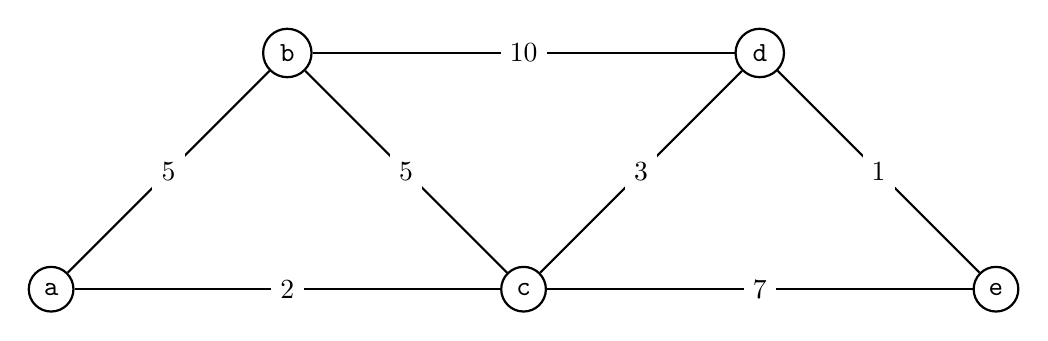
\begin{tikzpicture}[scale = 1.5]
\begin{scope}[every node/.style={circle,thick,draw}]
    \node (A) at (0,0) {\texttt{a}};
    \node (B) at (2,2) {\texttt{b}};
    \node (C) at (4,0) {\texttt{c}};
    \node (D) at (6,2) {\texttt{d}};
    \node (E) at (8,0) {\texttt{e}};
\end{scope}

\begin{scope}[every node/.style={fill=white,rectangle},
              every edge/.style={draw=black,thick}]
    % Undirected edges for MST (no arrows)
    \path (A) edge node {$5$} (B);
    \path (A) edge node {$2$} (C);
    \path (B) edge node {$5$} (C);
    \path (B) edge node {$10$} (D);
    \path (C) edge node {$3$} (D);
    \path (C) edge node {$7$} (E);
    \path (D) edge node {$1$} (E);
\end{scope}
\end{tikzpicture}
\end{center}

As you build the MST using Kruskal’s Algorithm, fill in the table below. 
For each step:

\begin{itemize}
  \item \textbf{Edge added:} Indicate the edge you selected for the MST in this step (e.g., $(\texttt{a},\texttt{b})$).
  \item \textbf{Vertices in MST:} List \textbf{all} vertices that are part of the MST \textbf{after} adding this edge.
\end{itemize}
You may not need all the rows.

\begin{longtable}{|>{\centering\arraybackslash}m{5cm}|>{\centering\arraybackslash}m{11cm}|}
\hline
\textbf{Edge Added} & \textbf{Vertices in MST} \\
\hline
\endfirsthead

\hline
\textbf{Edge added} & \textbf{Vertices in MST} \\
\hline
\endhead

\hline
\multicolumn{2}{r}{\small\itshape continued...} \\
\endfoot

\hline
\endlastfoot
& \\[3em]
\hline
 & \\[3em]
\hline
 & \\[3em]
\hline
 & \\[3em]
 \hline
 & \\[3em]
 \hline
 & \\[3em]
 \hline
 & \\[3em]
 \hline
 & \\[3em]
 \hline
 & \\[3em]
\end{longtable}

\newpage


\newpage

\subsection*{Question 2: Prim's Algorithm for MSTs}
\points[5] Run Prim's Algorithm to find the Minimum Spanning Tree (MST) on the graph below, with $v^{(0)} = \texttt{a}$.

\begin{center}

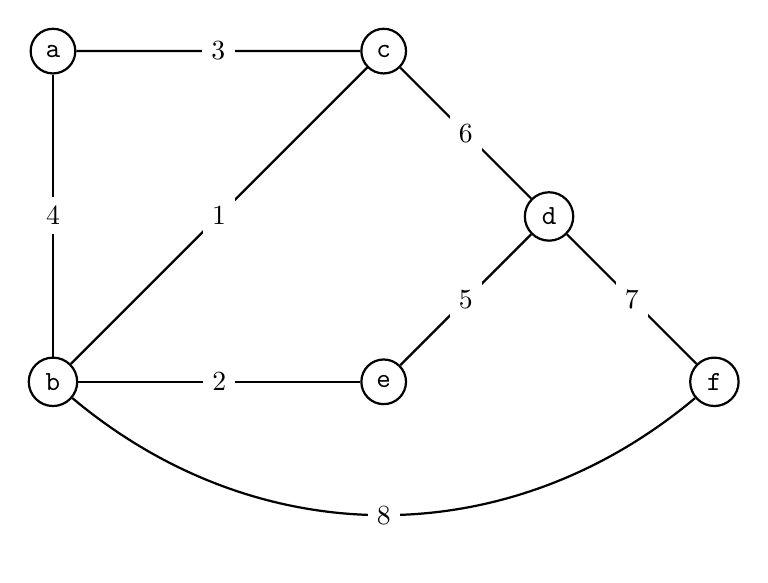
\begin{tikzpicture}[scale=1.4] 
\begin{scope}[every node/.style={circle,thick,draw}]
    \node (A) at (0,0) {\texttt{b}};
    \node (B) at (0,3) {\texttt{a}};
    \node (C) at (3,3) {\texttt{c}};
    \node (D) at (4.5,1.5) {\texttt{d}};
    \node (E) at (3,0) {\texttt{e}};
    \node (F) at (6,0) {\texttt{f}};
\end{scope}

\begin{scope}[every node/.style={fill=white,rectangle},
              every edge/.style={draw=black, thick}]
    \path (A) edge node {$4$} (B);
    \path (B) edge node {$3$} (C);
    \path (C) edge node {$6$} (D);
    \path (D) edge node {$5$} (E);
    \path (E) edge node {$2$} (A);
    \path (D) edge node {$7$} (F);
    \path [bend right=40] (A) edge node {$8$} (F);
    \path (C) edge node {$1$} (A);
\end{scope}
\end{tikzpicture}


\end{center}


Complete the table below step by step as you apply Prim’s Algorithm. In each row:

\begin{itemize}
\item \textbf{Edge added}:  Indicate the edge chosen at this step in the form \texttt{((u, v), w)}. 
    \item \textbf{Vertices in MST}: List \textbf{all} vertices that are currently included in the MST after each iteration. Begin with the starting vertex \(v^{(0)} = \texttt{a}\).



\item \textbf{Candidate edges}: After adding the new vertex to the MST, list all edges that connect any vertex currently in the MST to any vertex not yet in the MST.
Include each edge in the form $((\texttt{u}, \texttt{v}), \texttt{w})$, and sort them in order of increasing edge weight.
\newpage
\end{itemize}
You may not need all the rows.
\begin{longtable}{|>{\centering\arraybackslash}m{3cm}|>{\centering\arraybackslash}m{5cm}|>{\centering\arraybackslash}m{7cm}|}
\hline
\textbf{Edge added} & \textbf{Vertices in MST} & \textbf{Candidate edges} \\
\hline
\endfirsthead

\hline
\textbf{Edge added} & \textbf{Vertices in MST} & \textbf{Candidate edges} \\
\hline
\endhead

\hline
\multicolumn{3}{r}{\small\itshape continued...} \\
\endfoot

\hline
\endlastfoot

\raisebox{0pt}[3em][3em]{N/A} & \raisebox{0pt}[3em][3em]{\texttt{a}} & \\[-0.2em]
\hline
\raisebox{0pt}[3em][3em]{} & \raisebox{0pt}[3em][3em]{} & \\[-0.2em]
\hline
\raisebox{0pt}[3em][3em]{} & \raisebox{0pt}[3em][3em]{} & \\[-0.2em]
\hline
\raisebox{0pt}[3em][3em]{} & \raisebox{0pt}[3em][3em]{} & \\[-0.2em]
\hline
\raisebox{0pt}[3em][3em]{} & \raisebox{0pt}[3em][3em]{} & \\[-0.2em]
\hline
\raisebox{0pt}[3em][3em]{} & \raisebox{0pt}[3em][3em]{} & \\[-0.2em]
\hline
\raisebox{0pt}[3em][3em]{} & \raisebox{0pt}[3em][3em]{} & \\[-0.2em]
\hline
\raisebox{0pt}[3em][3em]{} & \raisebox{0pt}[3em][3em]{} & \\[-0.2em]
\hline
\raisebox{0pt}[3em][3em]{} & \raisebox{0pt}[3em][3em]{} & \\[-0.2em]
\hline
\raisebox{0pt}[3em][3em]{} & \raisebox{0pt}[3em][3em]{} & \\[-0.2em]

\end{longtable}





\newpage

\subsection*{Question 3: Union-Find}

\points[2]
Show the tree(s) that result after applying \texttf{union(e, y)} using \textbfinimum{union by rank}.  
Clearly indicate which root becomes the parent, explain why, and show the \textbf{updated rank} for the resulting tree.

\begin{center}
\qquad Rank 2 \qquad \qquad \qquad Rank 1
\end{center}

\begin{center}
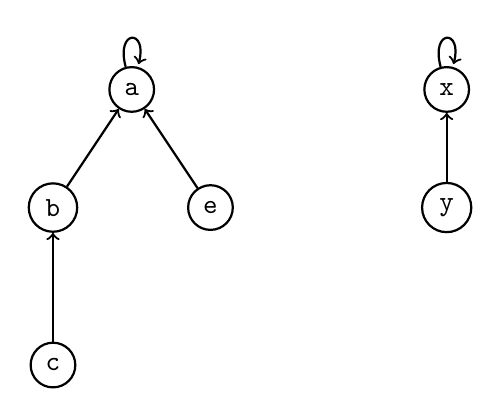
\begin{tikzpicture}[]
\begin{scope}[every node/.style={circle,thick,draw}]
    \node (A) at (1,3) {\texttt{a}};
    \node (B) at (0,1.5) {\texttt{b}};
    \node (C) at (0,-0.5) {\texttt{c}};
    \node (E) at (2,1.5) {\texttt{e}};
    \node (X) at (5,3) {\texttt{x}} ;
    \node (Y) at (5,1.5) {\texttt{y}} ;
\end{scope}

\begin{scope}[every node/.style={fill=white,circle},
              every edge/.style={draw=black, thick}]
    \path [->] (A) edge[loop above] (A);
    \path [->] (B) edge (A);
    \path [->] (C) edge (B);
    \path [->] (E) edge (A);
    \path [->] (X) edge[loop above] (X);
    \path [->] (Y) edge (X);
\end{scope}
\end{tikzpicture}
\end{center}

\newpage 


\points[2] Show the tree(s) that result after calling \texttt{find(g)} with \textbf{path compression}.  

\begin{center}
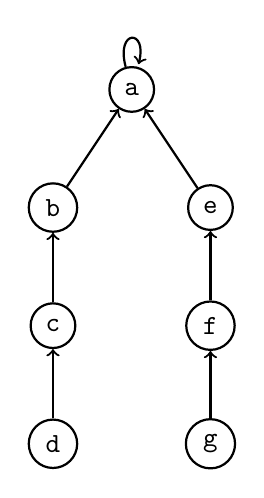
\begin{tikzpicture}
\begin{scope}[every node/.style={circle,thick,draw}]
    \node (A) at (1,3) {\texttt{a}};
    \node (B) at (0,1.5) {\texttt{b}};
    \node (C) at (0,0) {\texttt{c}};
    \node (D) at (0,-1.5) {\texttt{d}};
    \node (E) at (2,1.5) {\texttt{e}};
    \node (F) at (2,0) {\texttt{f}};
    \node (G) at (2,-1.5) {\texttt{g}};
\end{scope}

\begin{scope}[every node/.style={fill=white,circle},
              every edge/.style={draw=black, thick}]
    \path [->] (A) edge[loop above] (A);
    \path [->] (B) edge (A);
    \path [->] (C) edge (B);
    \path [->] (D) edge (C);
    \path [->] (E) edge (A);
    \path [->] (F) edge (E);
    \path [->] (G) edge (F);
\end{scope}
\end{tikzpicture}
\end{center}



\newpage

\subsection*{Question 4: Amortized Complexity Analysis}

\points[4] Consider a dynamic array that starts with a capacity of 1. 
Each time the array becomes full, it \textbf{triples} its capacity. 
Each \texttt{append()} operation costs 1 unit for inserting the new element, 
and each element copy during resizing also costs 1 unit.

\medskip

Given that the cost of the \( m \)-th \texttt{append} operation is defined as
\[
T(m) =
\begin{cases}
m, & \text{if } m \text{ is a power of } 3,\\[6pt]
1, & \text{otherwise.}
\end{cases}
\]

Find the total cost \( T(M) \) of performing \( M \) \texttt{append()} operations, and then compute the amortized cost per operation.


\newpage


\begin{center}
    \textit{(rough work - this page will not be marked)}
\end{center}
\clearpage

\end{document}